\subsection{obwohl und weil mit V2}

\begin{frame}
	{Schäfer \& Sayatz (wird Januar 2016 bei WLL eingereicht)}
	\begin{itemize}
	  \item Fragestellung: syntaktischer Status von \textit{obwohl} und \textit{weil}\\mit V2 -- insbesondere \alert{Integriertheit}
	  \item klassisch: Battle Reis (z.\,B.\ 2013) vs.\ Antomo \& Steinbach (z.\,B.\ 2010, 2013)
	  \item empirisches Problem: Tests auf Integriertheit\\sind nicht operationalisierbar
	  \item Experimente: kostspielig und kompliziert
	  \item hier wird nur die \alert{graphematische Seite} betrachtet
	\end{itemize}
\end{frame}

\begin{frame}
	{Korpusstudie}
	\begin{itemize}
		\item DECOW12Q: spontansprachliches Korpus\\(Heuristik basierend auf Schäfer \& Sayatz 2014)
		\item je 5.000 Belege für \textit{obwohl} und \textit{weil}
		\item \textit{obwohl}: ca.\ 6\% mit V2
		\item \textit{weil}: ca.\ 7\% mit V2
		\item deutlich anders als Standard-Schriftsprache,\\deutlich anders als gesprochene Sprache
		\item aufwändigere Analyse mit GLMs
		\item \alert{natürlich} werden die Daten mit der Einreichung\\auf meiner Webseite veröffentlicht
	\end{itemize}
\end{frame}

\begin{frame}
	{Interpretation}
	\centering
	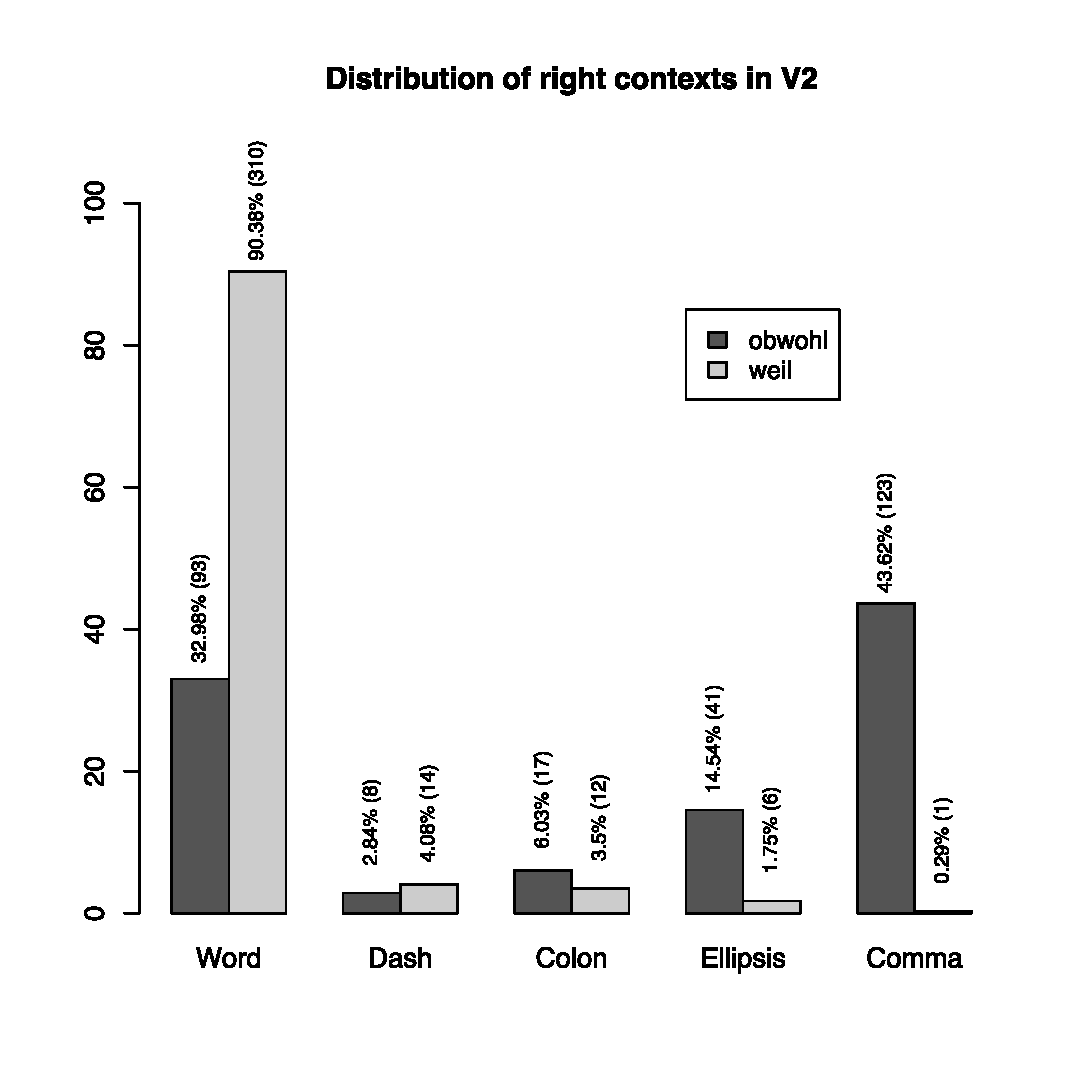
\includegraphics[height=0.9\textheight]{v2_right}
\end{frame}

\begin{frame}
	{Interpretation}
	\centering
	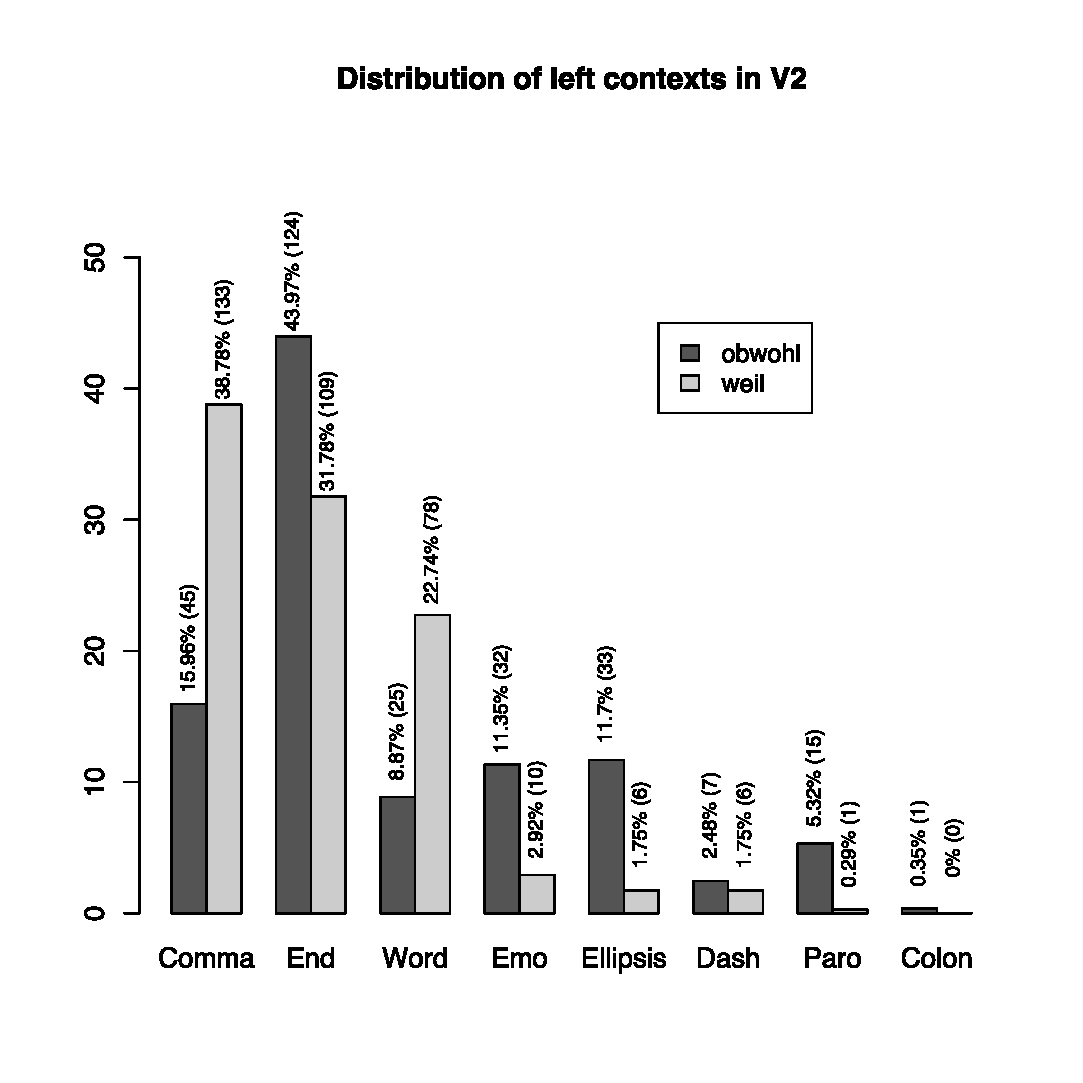
\includegraphics[height=0.9\textheight]{v2_left}
\end{frame}

